\documentclass{beamer}

\usecolortheme[light]{solarized}

\beamertemplatenavigationsymbolsempty
\setbeamertemplate{frametitle}[default][center]

\usepackage{hyperref}
\usepackage{minted}

\usepackage{graphicx}
\usepackage{tikz}

\usetikzlibrary{calc, patterns}

\begin{document}

    \begin{frame}
        \begin{center}
            \Huge

            Modelling epidemics with Python

            \Large
            \vspace{1cm}
            \href{https://twitter.com/drvinceknight}{@drvinceknight}\\
            \url{vknight.org}\\
            \texttt{knightva@cardiff.ac.uk}
        \end{center}


    \end{frame}

    \begin{frame}
        \begin{center}
            \Large
            Not Me
        \pause
        \vspace{1cm}

        
\includegraphics[height=.7\textheight]{static/fauci.jpg}

        \end{center}
    \end{frame}

    \begin{frame}
        \centering

        
\includegraphics[height=.4\textheight]{static/CUident_CMYK.eps}
        \hfill
        
\includegraphics[height=.4\textheight]{static/pyconuk.jpg}

        \vspace{.1\textheight}

        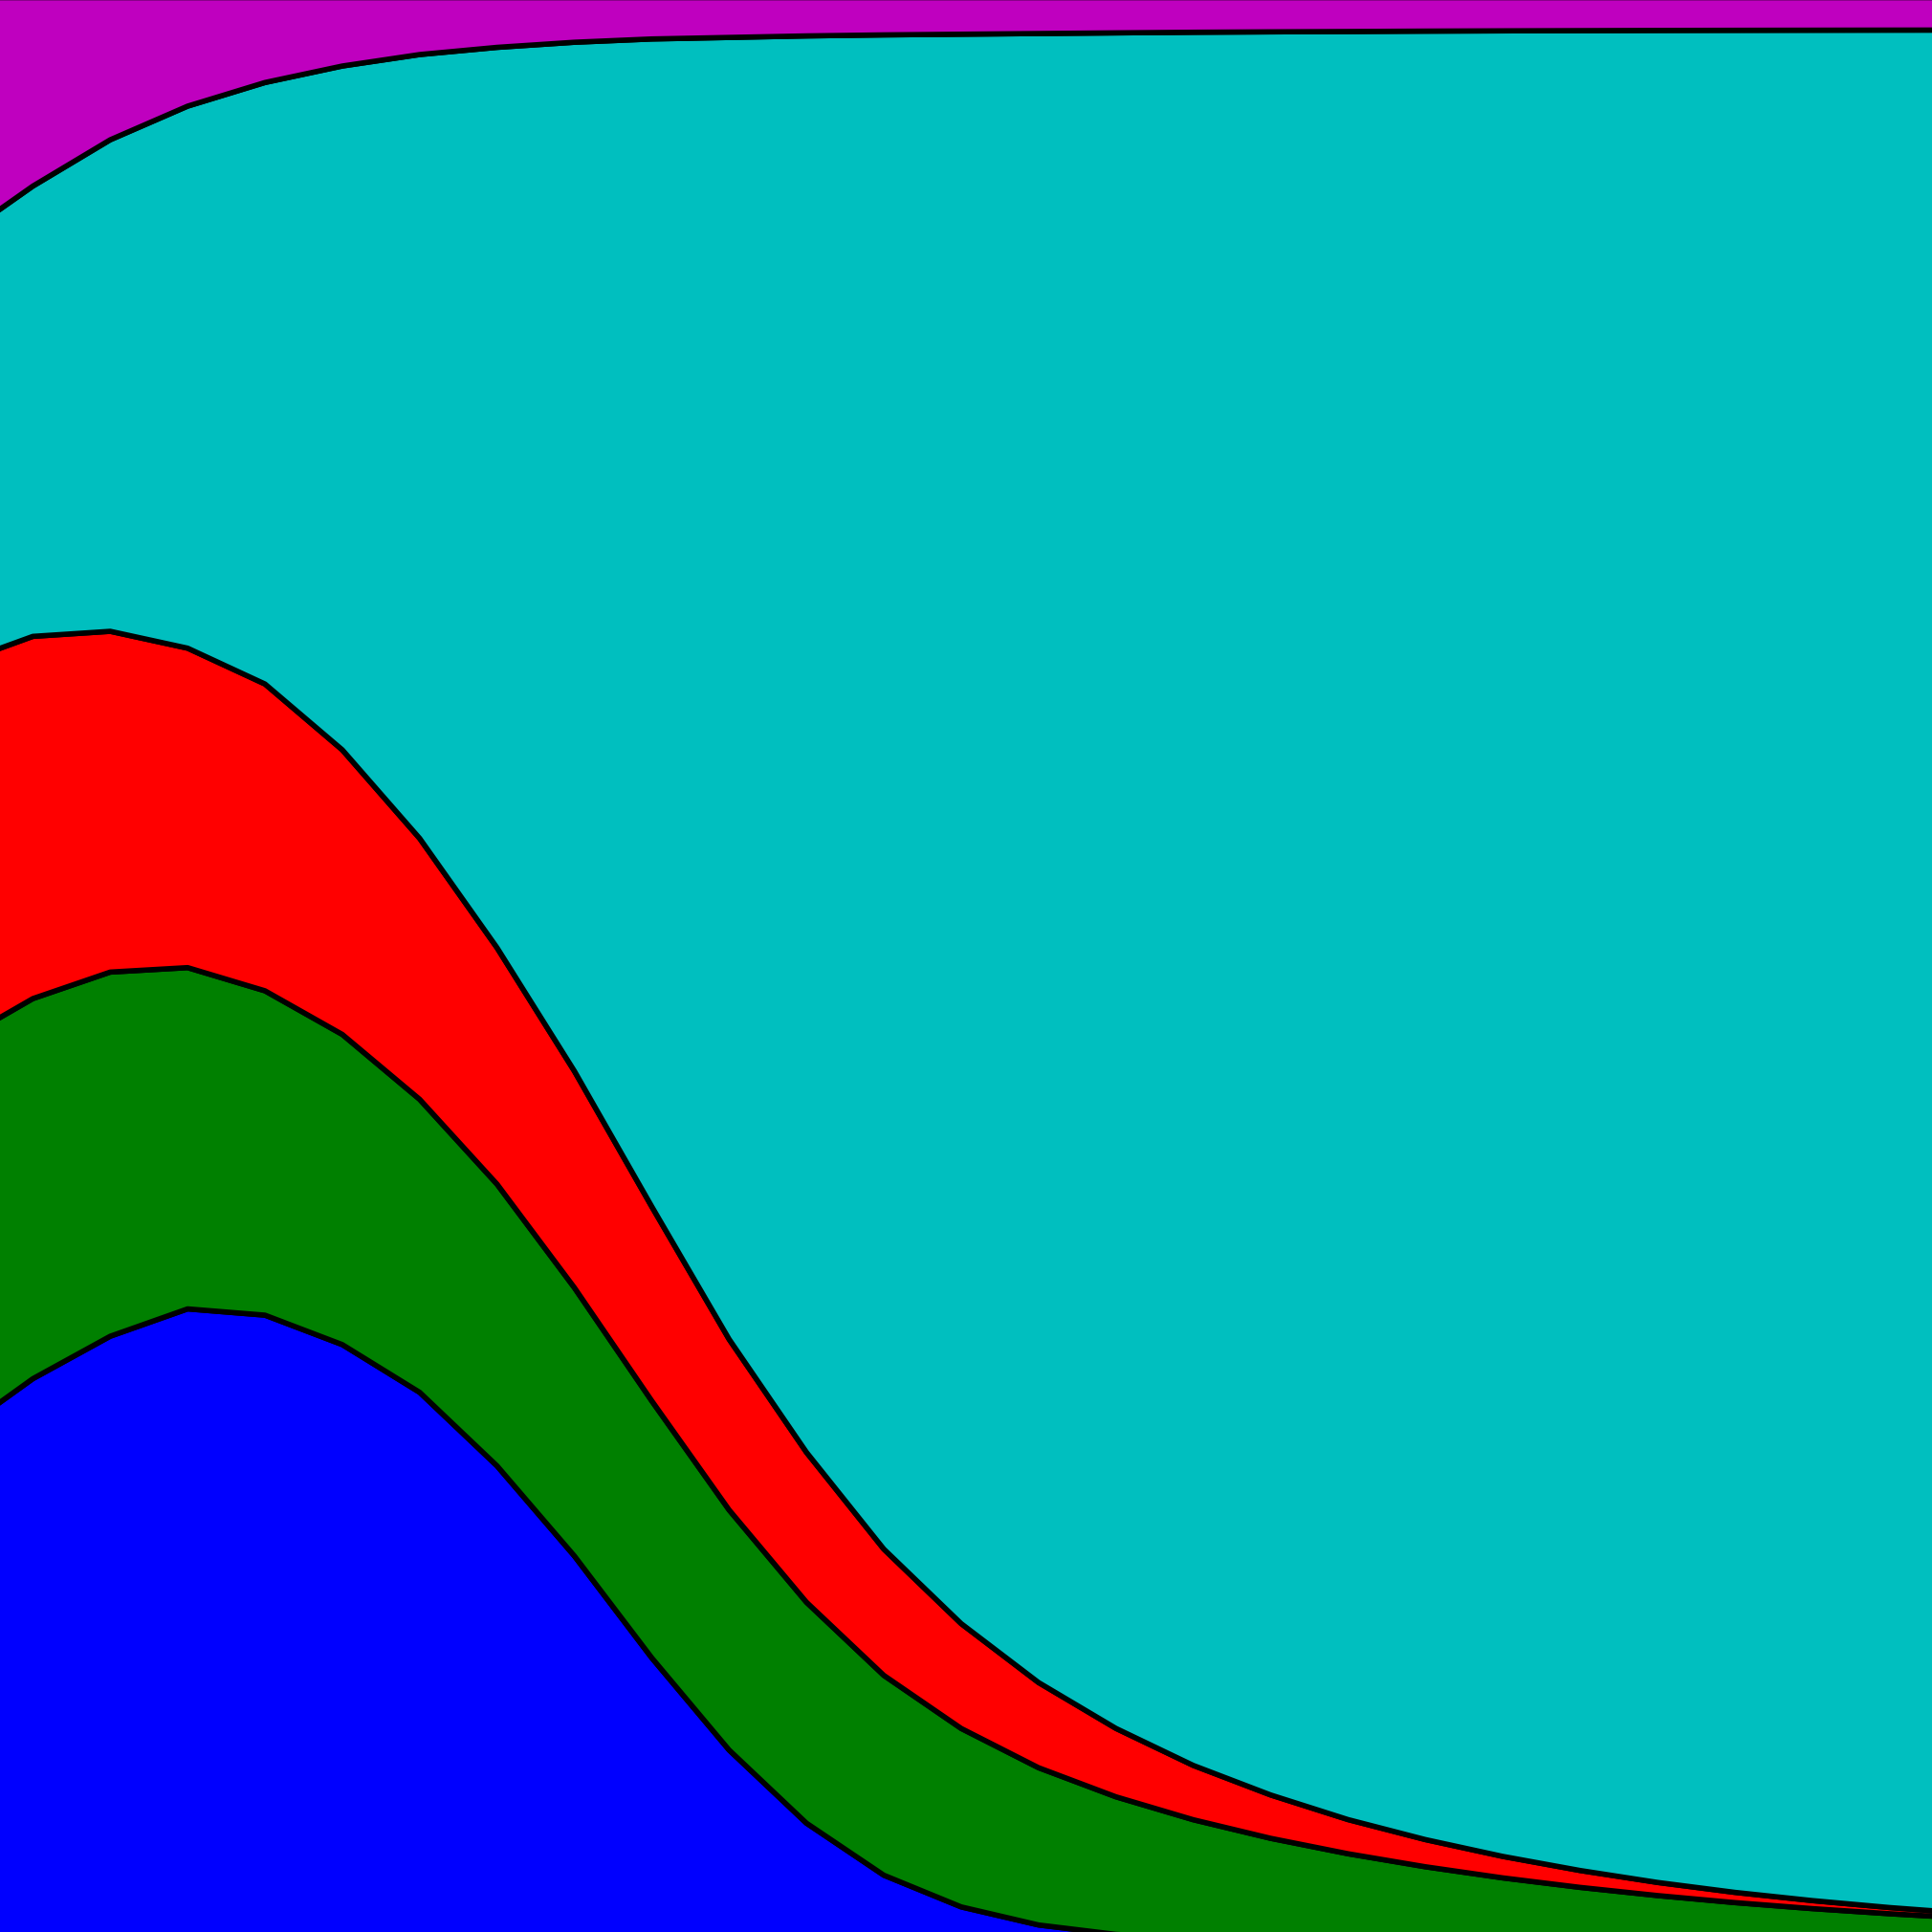
\includegraphics[height=.4\textheight]{static/axelrod_logo.png}
        \hfill
        
\includegraphics[height=.4\textheight]{static/ssi-logo.png}
    \end{frame}

    \begin{frame}
        \begin{center}
            \includegraphics[width=.95\textwidth]{static/pycon-namibia-2018.jpg}
        \end{center}
    \end{frame}

    \begin{frame}
        \begin{center}
            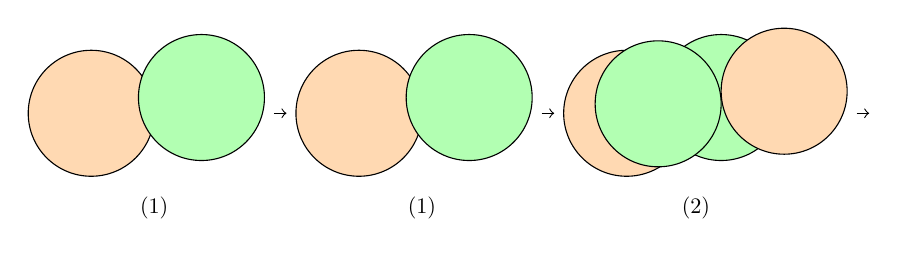
\begin{tikzpicture}[scale=.8, transform shape]
                \draw [fill=orange!30] (0, 0) circle (1);
                \draw [fill=green!30] (1.75, .25) circle (1);

                \node at (1, -1.5) {(1)};

                \draw [->] (2.9, 0) -- (3.1, 0);

                \draw [fill=orange!30] (4.25, 0) circle (1);
                \draw [fill=green!30] (6, .25) circle (1);

                \node at (5.25, -1.5) {(1)};


                \draw [->] (7.15, 0) -- (7.35, 0);

                \draw [fill=orange!30] (8.5, 0) circle (1);
                \draw [fill=green!30] (10, .25) circle (1);
                \draw [fill=green!30] (9, .15) circle (1);
                \draw [fill=orange!30] (11, .35) circle (1);

                \node at (9.6, -1.5) {(2)};

                \draw [->] (12.15, 0) -- (12.35, 0);
            \end{tikzpicture}

        \LARGE
        \[
            x_n =
            \begin{cases}
                1\;&\text{ if }n\in\{0, 1\}\\
                x_{n-1} + x_{n-2}
            \end{cases}
        \]
        \end{center}
    \end{frame}

    \begin{frame}
        \begin{center}
            \begin{tikzpicture}
                \node [draw, fill=blue!20] (start) at (0, 0) {};
                \node [draw, fill=blue!20] (finish) at (10, 0) {};
                \draw [->] (start) -- (finish);

                \draw ($(start) + (3, .1)$) circle (.1);
                \draw ($(start) + (3.5, .1)$) circle (.1);
                \draw (3, .2) -- (3, .5) -- (3.5, .2) -- cycle;


                \draw [<->] (0, -1) -- (3.5, -1) node [below] {3.5};
                \draw [<->] (0, -2) -- (10, -2) node [below] {10};
            \end{tikzpicture}

        \Huge

        \[3.5 + x = 10\]
        \end{center}
    \end{frame}



    \begin{frame}
        \begin{center}
            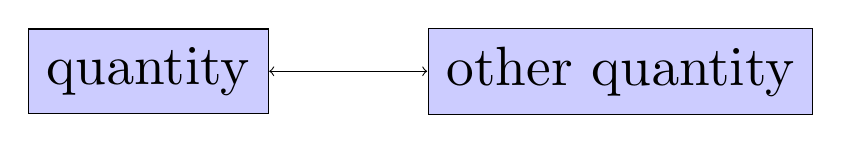
\begin{tikzpicture}[scale=2, transform shape]
                \node [draw, fill=blue!20] (quantity) at (0, 0) {quantity};
                \node [draw, fill=blue!20] (other_quantity) at (3, 0) {other quantity};
                \draw [<->] (quantity) -- (other_quantity);
            \end{tikzpicture}
        \end{center}
    \end{frame}

    \begin{frame}
            \begin{tikzpicture}
                \node [draw, fill=blue!20] (start) at (0, 0) {};
                \node [draw, fill=blue!20] (finish) at (10, 0) {};
                \draw [->] (start) -- (finish);

                \draw ($(start) + (3, .1)$) circle (.1);
                \draw ($(start) + (3.5, .1)$) circle (.1);
                \draw (3, .2) -- (3, .5) -- (3.5, .2) -- cycle;


                \draw [<->] (0, -1) -- (3.5, -1) node [below] {3.5};
                \draw [<->] (0, -2) -- (10, -2) node [below] {10};
            \end{tikzpicture}
    \end{frame}

    \begin{frame}
        \begin{center}
            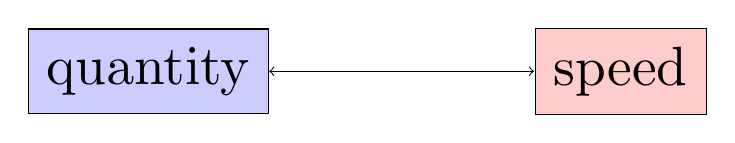
\begin{tikzpicture}[scale=2, transform shape]
                \node [draw, fill=blue!20] (quantity) at (0, 0) {quantity};
                \node [draw, fill=red!20] (other_quantity) at (3, 0) {speed};
                \draw [<->] (quantity) -- (other_quantity);
            \end{tikzpicture}
        \end{center}
    \end{frame}

    \begin{frame}
        \begin{center}
            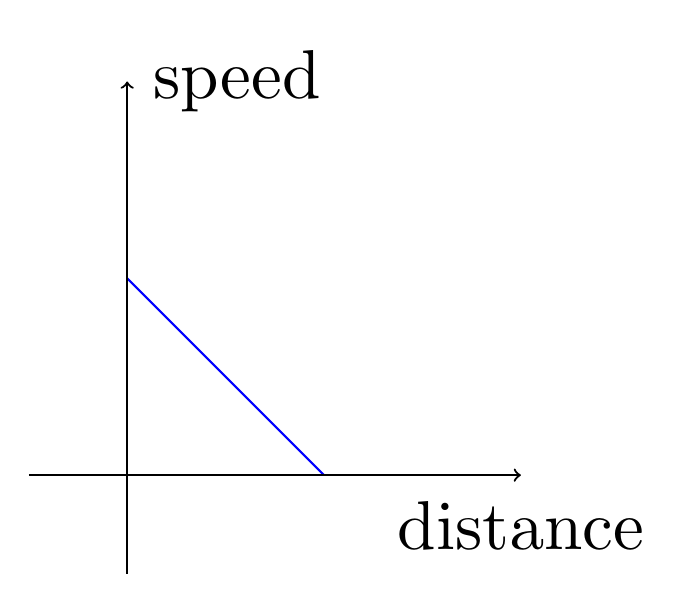
\begin{tikzpicture}[scale=2.5, transform shape]
                \draw[domain=0:1, color=blue, thick] plot (\x, {1 - \x});
                \draw [thick, ->] (-0.5,0) -- (2,0) node [below] {distance};
                \draw [thick, ->] (0,-.5) -- (0,2) node [right] {speed};
            \end{tikzpicture}
        \end{center}
    \end{frame}


    \begin{frame}
        \begin{center}
            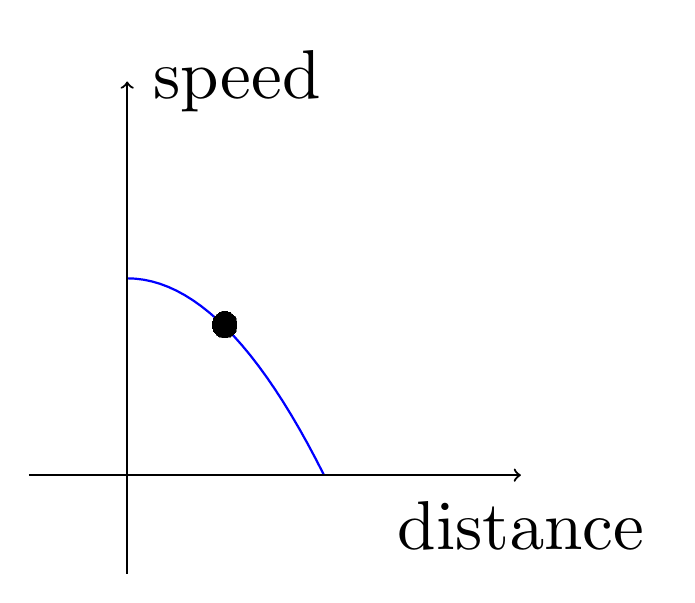
\begin{tikzpicture}[scale=2.5, transform shape]
                \draw[domain=0:1, color=blue, thick] plot (\x, {1 - (\x)^2});
                \draw [thick, ->] (-0.5,0) -- (2,0) node [below] {distance};
                \draw [thick, ->] (0,-.5) -- (0,2) node [right] {speed};
                \pause
                \node at (.5,.75) {\textbullet};
            \end{tikzpicture}
        \end{center}
    \end{frame}


    \begin{frame}
        \Huge
        \begin{center}
            Coffee break.
        \end{center}
    \end{frame}

    \begin{frame}
        \Huge
        \[
            \frac{dT}{dt} = K (T_{\text{room} - T(t)})
        \]
    \end{frame}

    \begin{frame}
        \Huge
        \begin{center}
            \texttt{import sympy}
        \end{center}
    \end{frame}

    \begin{frame}
        \begin{center}
            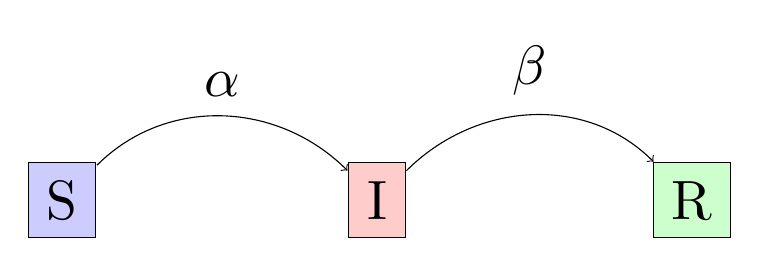
\begin{tikzpicture}[scale=2, transform shape]
                \node [draw, fill=blue!20] (S) at (0, 0) {S};
                \node [draw, fill=red!20] (I) at ($(S) + (2, 0)$) {I};
                \node [draw, fill=green!20] (R) at ($(I) + (2, 0)$) {R};

                \draw [->] (S) edge [out=45, in=135] node [above] {\(\alpha\)} (I);
                \draw [->] (I) edge [out=45, in=135] node [above] {\(\beta\)} (R);
            \end{tikzpicture}
        \end{center}
        \pause
        \Large
        \[\frac{dS}{dt} = - \alpha I S\qquad
          \frac{dI}{dt} =  \alpha I S - \beta I\qquad
          \frac{dR}{dt} =  \beta I
         \]
    \end{frame}

    \begin{frame}
        \Huge
        \begin{center}
            \texttt{import scipy}
        \end{center}
    \end{frame}

    \begin{frame}
        \begin{center}
            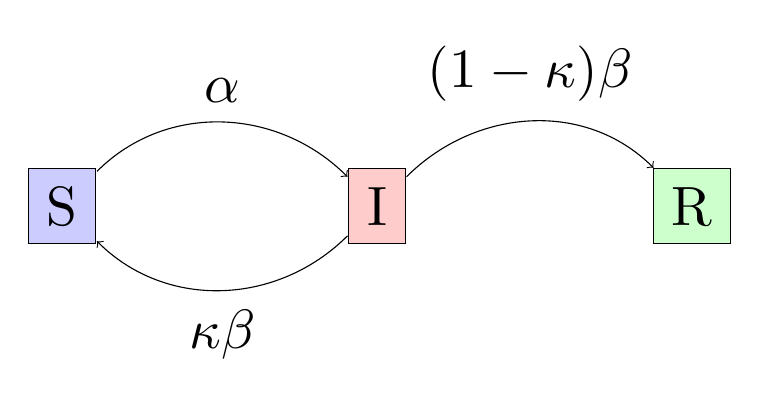
\begin{tikzpicture}[scale=2, transform shape]
                \node [draw, fill=blue!20] (S) at (0, 0) {S};
                \node [draw, fill=red!20] (I) at ($(S) + (2, 0)$) {I};
                \node [draw, fill=green!20] (R) at ($(I) + (2, 0)$) {R};

                \draw [->] (S) edge [out=45, in=135] node [above] {\(\alpha\)} (I);
                \draw [->] (I) edge [out=45, in=135] node [above] {\((1-\kappa)\beta\)} (R);
                \draw [->] (I) edge [out=-135, in=-45] node [below] {\(\kappa\beta\)} (S);
            \end{tikzpicture}
        \end{center}
        \pause
        \Large
        \[\frac{dS}{dt} = - \alpha I S + \kappa \beta I \qquad
          \frac{dI}{dt} =  \alpha I S - \beta I\qquad
          \frac{dR}{dt} =  (1 - \kappa) \beta I
         \]
    \end{frame}

    \begin{frame}
        \begin{center}
            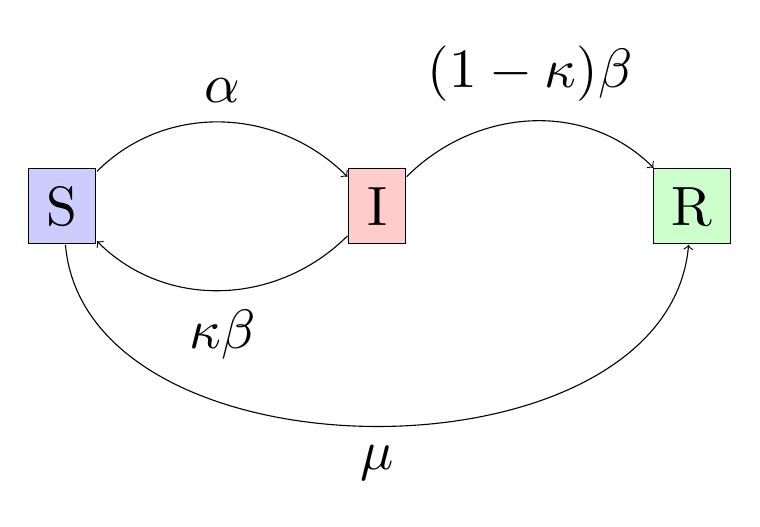
\begin{tikzpicture}[scale=2, transform shape]
                \node [draw, fill=blue!20] (S) at (0, 0) {S};
                \node [draw, fill=red!20] (I) at ($(S) + (2, 0)$) {I};
                \node [draw, fill=green!20] (R) at ($(I) + (2, 0)$) {R};

                \draw [->] (S) edge [out=45, in=135] node [above] {\(\alpha\)} (I);
                \draw [->] (I) edge [out=45, in=135] node [above] {\((1-\kappa)\beta\)} (R);
                \draw [->] (I) edge [out=-135, in=-45] node [below] {\(\kappa\beta\)} (S);
                \draw [->] (S) edge [out=-85, in=-95] node [below] {\(\mu\)} (R);
            \end{tikzpicture}
        \end{center}
        \pause
        \large
        \[\frac{dS}{dt} = - \alpha I S + \kappa \beta I - \mu S\qquad
          \frac{dI}{dt} =  \alpha I S - \beta I\qquad
          \frac{dR}{dt} =  (1 - \kappa) \beta I + \mu S
         \]
    \end{frame}

    \begin{frame}
        \begin{center}
            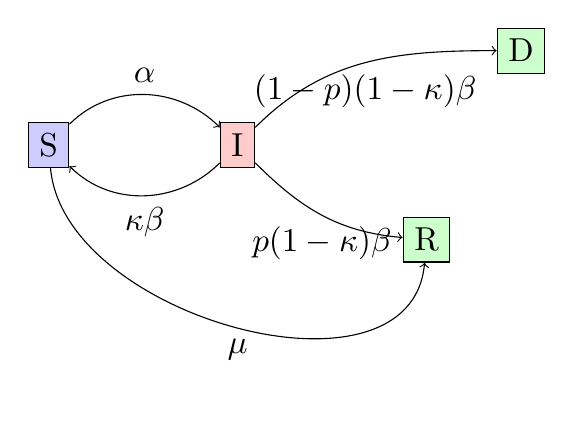
\begin{tikzpicture}[scale=1.2, transform shape]
                \node [draw, fill=blue!20] (S) at (0, 0) {S};
                \node [draw, fill=red!20] (I) at ($(S) + (2, 0)$) {I};
                \node [draw, fill=green!20] (D) at ($(I) + (3, 1)$) {D};
                \node [draw, fill=green!20] (R) at ($(I) + (2, -1)$) {R};

                \draw [->] (S) edge [out=45, in=135] node [above] {\(\alpha\)} (I);
                \draw [->] (I) edge [out=-45, in=175] node [below] {\(p(1-\kappa)\beta\)} (R);
                \draw [->] (I) edge [out=45, in=180] node [below] {\((1-p)(1-\kappa)\beta\)} (D);
                \draw [->] (I) edge [out=-135, in=-45] node [below] {\(\kappa\beta\)} (S);
                \draw [->] (S) edge [out=-85, in=-95] node [below] {\(\mu\)} (R);
            \end{tikzpicture}
        \end{center}
        \pause
        \large
        \[\frac{dS}{dt} = - \alpha I S + \kappa \beta I - \mu S\qquad
            \frac{dI}{dt} =  \alpha I S - \beta I\]
         \[
          \frac{dR}{dt} = p (1 - \kappa) \beta I + \mu S\qquad
          \frac{dD}{dt} = (1 - p) (1 - \kappa) \beta I 
         \]
    \end{frame}

    \begin{frame}
        \begin{itemize}
            \item \texttt{sympy}: powerful python library for symbolic
                mathematics;
            \item \texttt{scipy.integrate.odeint}: numerical integration for
                numerical solutions of differential equations.
        \end{itemize}

        \vspace{1cm}

        \begin{center}
            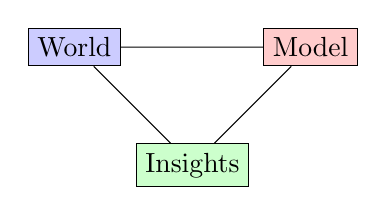
\begin{tikzpicture}
                \node (world) [draw, fill=blue!20] at (0, 0) {World};
                \node (model) [draw, fill=red!20] at (3, 0) {Model};
                \node (insights) [draw, fill=green!20]  at (1.5, -1.5) {Insights};

                \draw (world) -- (model) -- (insights) -- (world);
            \end{tikzpicture}
        \end{center}
    \end{frame}

    \begin{frame}
        \begin{center}
            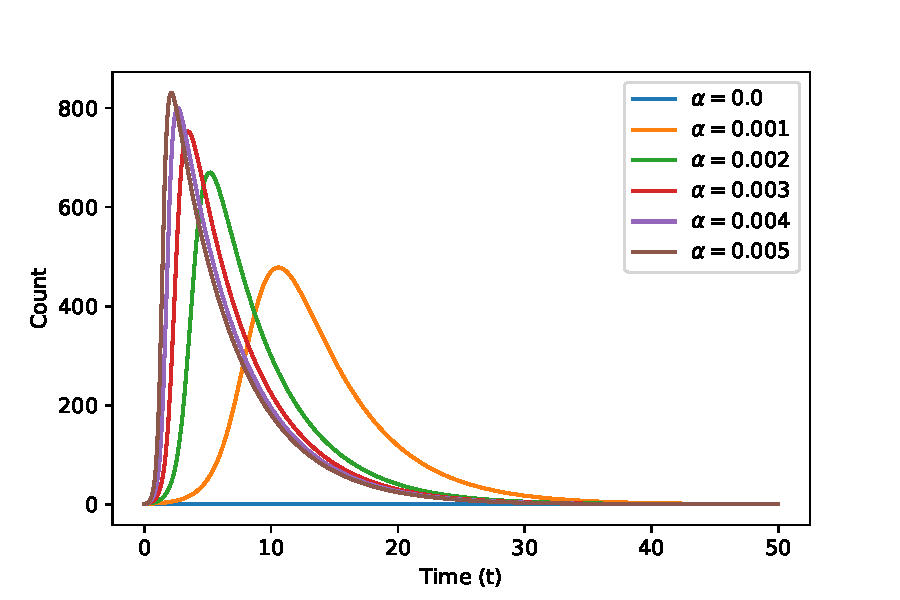
\includegraphics[width=.95\textwidth]{./static/flatting_of_curve.pdf}
        \end{center}
    \end{frame}

    \begin{frame}
        \Huge
        \begin{center}
            \href{https://twitter.com/drvinceknight}{@drvinceknight}\\
            \url{vknight.org}\\
            \texttt{knightva@cardiff.ac.uk}
        \end{center}
    \end{frame}

\end{document}
